\documentclass{article}
\usepackage{graphicx}
\usepackage{textgreek}

\begin{document}
\title{Spécifiation de conception de la base de données : Jalon 1}

\author{Louis-Vincent CAPELLI \and Alexandre THEISSE \and Tom SARTORI \and Raphaël TURCOTTE}
\date{\today}
\maketitle
\newpage

\tableofcontents
\newpage

\section{Introduction}
\subsection*{Objet de portée du document}
Ce document a pour but de décrire les modifications à apporter à la base de données
SSQA afin de répondre aux exigences formulées dans la
spécifiation des exigences du modèle.
Il s'adresse à toute personne qui pourrait avoir à travailler sur la base de données
SSQA à l'avenir.

\section{Présentation générale du résultat}
\subsection{Schéma modifié}
Voici ci-après le schéma modifié de la base de données SSQA. Il est en de
nombreux points similaire au schéma préliminaire, mais comporte des modifications
importantes, notamment au niveau de la représentation des unités et de la gestion
de la validité des mesures. Ces modifications sont décrites plus en détail dans
la suite du document, à la lumière des différentes exigences.

\begin{figure}[h]
\centering
\caption{Schéma modifié}
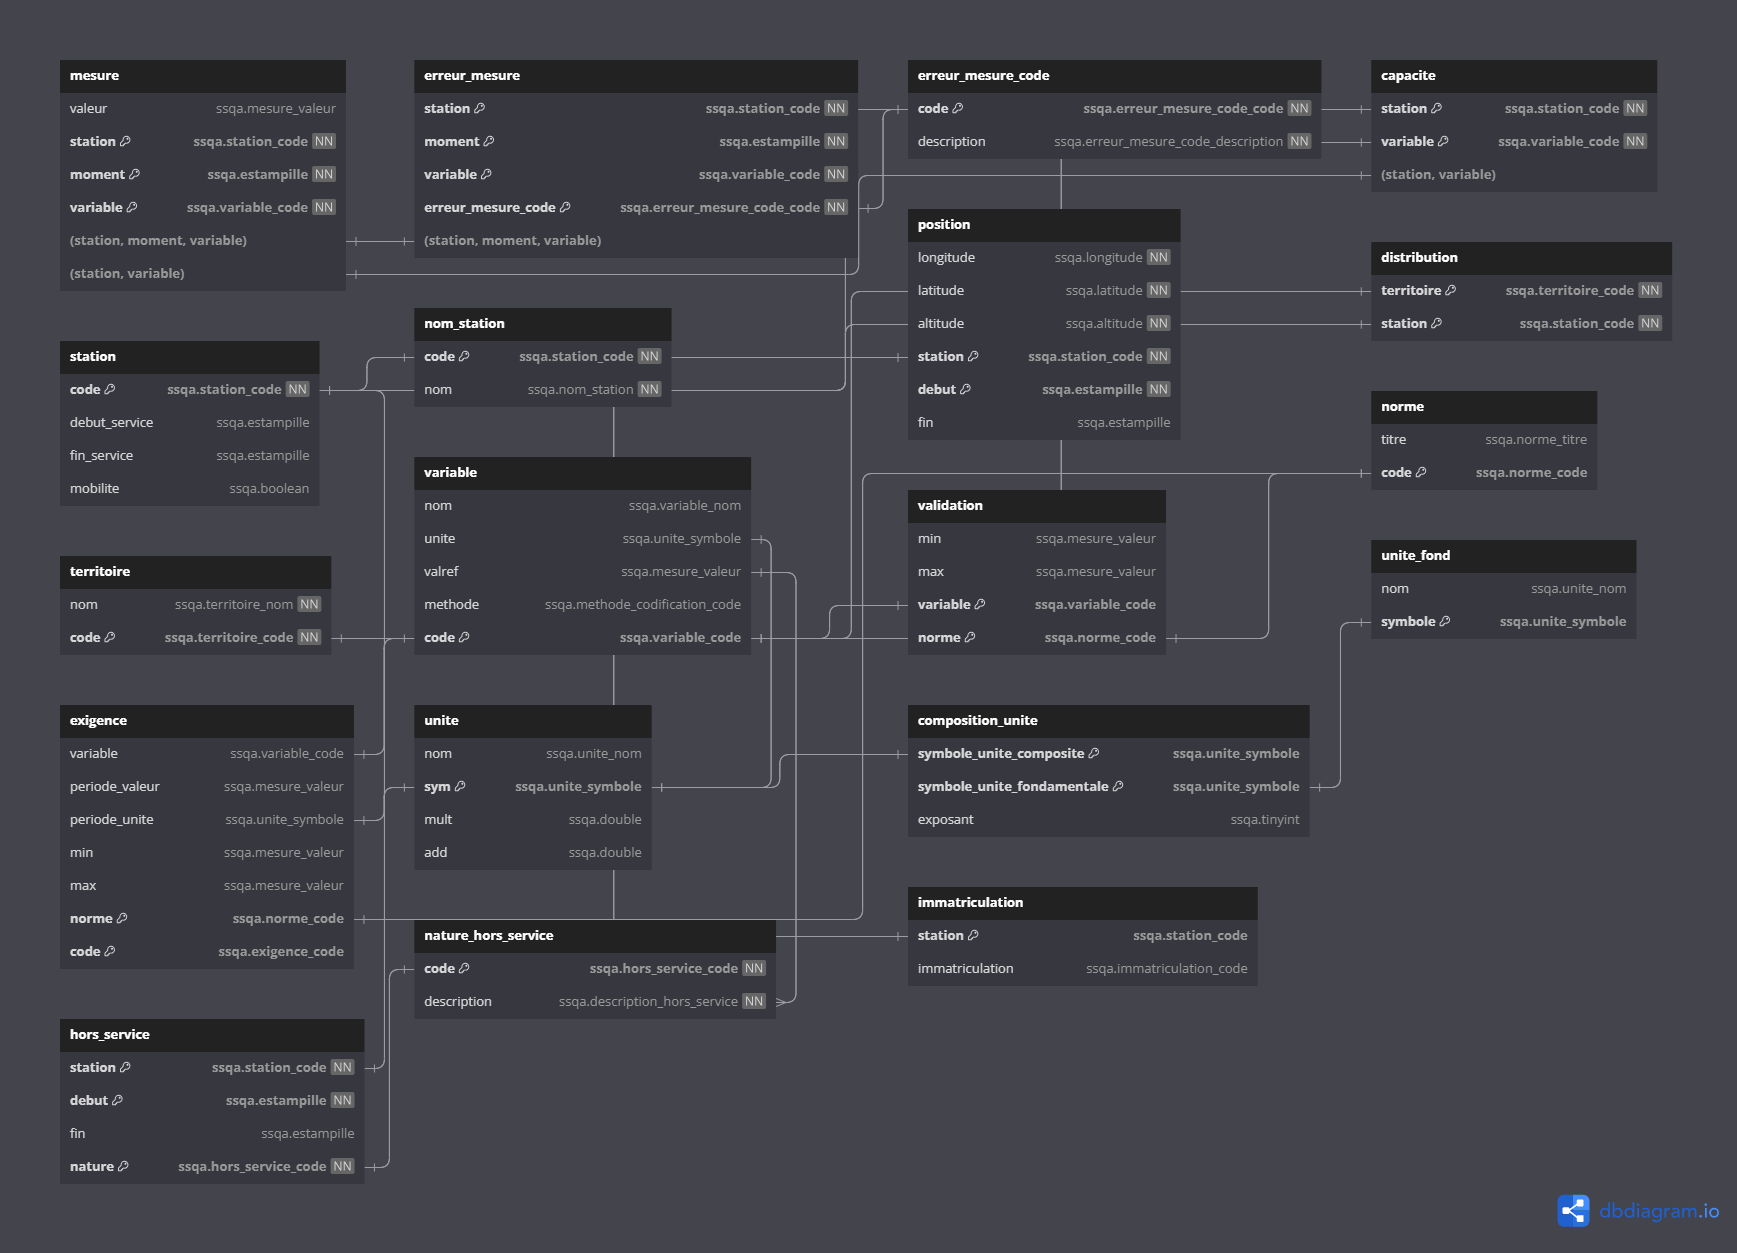
\includegraphics[scale=0.24]{modif.png}
\end{figure}

\subsection{Normalisation}
Le schéma modifié, après avoir été mis au point était déjà en forme normale de 
Boyce-Codd. 
Nous avons décidé de nous assurer qu'il était également en 5NF.
Les relations de comprenant pas au moins un attribut non-clé sont (toutes les autres sont automatiquement en 5NF) :
\begin{itemize}
    \item Capacité : qui est en 5NF car elle ne contient que deux attributs.
    \item Distribution : qui est en 5NF car elle ne contient que deux attributs.
    \item Erreur\_mesure : si on la décompose la relation Erreur\_mesure(station, moment, variable, erreur\_mesure\_code)
en quatre sous-relations à trois éléments :
    \begin{itemize}
        \item (station, moment, variable)
        \item (station, moment, erreur\_mesure\_code)
        \item (station, variable, erreur\_mesure\_code)
        \item (moment, variable, erreur\_mesure\_code)
    \end{itemize}
on perd de l'information. Par exemple :
    \begin{itemize}
        \item Station 1, 1/1/1970, concentration NO2 (peut être une erreur de manipulation)
        \item Station 1, 1/1/1970, capteur surchauffe (peut être sur la concentration en CO2)
        \item Station 1, concentration NO2, capteur surchauffe (peut être le 2/1/1970)
        \item 1/1/1970, concentration NO2, capteur surchauffe (peut être dans la Station 2)
    \end{itemize}
On ne peut pas déduire de ces 4 tuples que "Station 1, 1/1/1970, concentration NO2, capteur surchauffe" donc on n'a pas à décomposer la table.
\end{itemize}


\section{Choix de conception}
\subsection{R01.SI\_mod}
\paragraph{Description} Représenter toutes les unités en fonction des unités fondamentales définies par le SI
et de deux coefficients additif et multiplicatif.

\paragraph{Solution choisie}
Une unité est modélisée par un symbole et un nom. Sa définition est complétée par une valeur de multiplication et une valeur d'addition par rapport à l'unité fondamentale associée.
Une table Unité\_fondamentale permet de définir les unités fondamentales du SI (et d'en ajouter si nécessaire).
Une table Composition\_unité permet de définir les unités composées à partir des unités fondamentales, chaque entrée de cette table est composée d'une unité fondamentale et d'un exposant
et référence l'unité correspondante.
Si l'unité est fondamentale, alors la valeur de multiplication est 1 et la valeur d'addition est 0 et elle n'est représentée que par une seule entrée dans la table Composition\_unité.

\paragraph{Solution alternative}
Nous avions pensé à une autre solution pour représenter les unités comme le radian.
Actuellement, le radian est ajouté comme unité fondamentale,
mais nous aurions pu également ajouter toutes les unités du SI en double dans la table
Unité\_fondamentale, afin de pouvoir les utiliser avec deux exposants différents
dans la table Composition\_unité. Cela aurait permis de représenter le radian
comme une unité composée de mètre et de mètre, et ainsi d'être plus cohérent avec
la définition du SI. Cependant, cette solution aurait été plus lourde à mettre en
place et moins facile à comprendre. Nous avons donc préféré la solution actuelle qui
permet les mêmes fonctionnalités.

\subsection{R02.SI\_sym}
\paragraph{Description} Restreindre les symboles des unités grace aux règles du BIPM.

\paragraph{Solution choisie}
Nous n'avons pas implémenté cette exigence car nous n'avons pas trouvé de règles
claires pour les symboles des unités. En supposant que l'utilisateur 
peut créer de nouvelles unités à volonté, il est impossible de prévoir la forme des symboles.
Dans les exemples fournis avec le schéma préliminaire de l'EPP\_V1, l'une des unités
avait pour symbole \textmugreek g/m3, mais on peut très bien imaginer des unités plus complexes avec
des symboles comme \textmugreek g*s2*A/m3.

\subsection{R03.Validation\_nom}
\paragraph{Description} Changer le nom de la table "Seuils" pour "Validation"
et faire percoler les conséquences de ce changement dans le reste de la base de données.

\paragraph{Solution choisie}
Nous avons renommé la table Seuils en Validation et modifié les noms des contraintes
correspondantes.

\subsection{R04.Variable\_contrainte}
\paragraph{Description} 
\begin{itemize}
    \item Vérifier que la valeur de référence de la variable est comprise dans l'intervalle de
    validité fixé par la norme associée.
    \item Vérifier que les min et max des exigences pour une variable sont compris
    dans l'intervalle de validité fixé par la norme associée pour cette variable.
\end{itemize}

\paragraph{Solution choisie}
Nous avons crée un trigger qui vérifie, avant l'insertion dans la table Validation,
que la valeur de référence de la variable est comprise dans l'intervalle de validité.
Si ce n'est pas le cas, l'insertion est refusée et l'erreur "L'intervalle de validation est invalide"
est renvoyée.

Nous avons aussi crée un trigger qui vérifie, avant l'insertion dans la table Exigence,
que les min et max sont compris dans l'intervalle de validité pour la variable et la norme
concernées. Si ce n'est pas le cas, l'insertion est refusée et l'erreur "La valeur minimale de l'exigence est invalide"
ou l'erreur "La valeur maximale de l'exigence est invalide" est renvoyée selon le cas.

\subsection{R05.Méthode\_codification}
\paragraph{Description} Les méthodes d'échantillonnage des variables sont en texte libre, ce qui laisse place à des erreurs de saisie qui
pourraient résulter en la définition de plusieurs représentations pour une même méthode. Afin de mieux valider les données, les méthodes devraient être codifiées.

\paragraph{Solution choisie}
Nous avons considéré que les méthodes d'échantillonnage n'étaient pas censées
évoluer dans le temps, et qu'il n'était donc pas nécessaire de pouvoir
en ajouter de nouvelles. Nous avons donc décidé de changer le type de la
colonne en un type enum, qui permet de restreindre les valeurs possibles
à une liste prédéfinie.

\paragraph{Solution alternative}
Nous aurions pu également créer une table Méthode\_échantillonnage qui
aurait référencé les méthodes possibles, et qui aurait été référencée
par la table Variable. Cela aurait permis de pouvoir ajouter de nouvelles
méthodes d'échantillonnage à l'avenir.

\subsection{R06.Station\_service}
\paragraph{Description} Afin de permettre de valider les temps des mesures :
ajouter les attributs de mise en exploitation et de fin d'exploitation de la station et 
maintenir une table des périodes d'entretien ou de non-disponibilité des stations.

\paragraph{Solution choisie}
Nous avons créé des tables Nature\_hors\_service et Hors\_service qui permettent
de définir les périodes d'indisponibilité des stations. La table Hors\_service
référence la table Nature\_hors\_service et la table Station. Elle contient
également une date de début et une date de fin. La table Nature\_hors\_service
contient un nom et une description et permet de définir les différentes
raisons pour lesquelles une station peut être indisponible de manière 
évolutive au cours du temps.

Nous avons également ajouté une date de mise en exploitation et une date de fin
d'exploitation à la table Station sous la forme de deux nouveaux attributs de type
Estampille.

\subsection{R07.Station\_mobilité}
\paragraph{Description} Certaines stations sont mobiles, leurs coordonnées varient donc dans le temps. Les stations fixes peuvent aussi
être déplacées à l'occasion. Ainsi il faudra modifier le schéma afin 
de pouvoir consigner l'évolution des coordonnées des stations.

\paragraph{Solution choisie}
Nous avons ajouté un attribut mobilite de type booléen à la table Station qui permet de savoir
si une station est mobile ou non.

Nous avons créé une table Position qui référence la table Station et qui contient
des dates de début et de fin, ainsi que des coordonnées. La table Position permet
de définir les différentes positions qu'une station peut occuper au cours du temps.

Nous avons ainsi transféré les attributs latitude, longitude et altitude de la table Station
vers la table Position en ajoutant les tuples correspondants aux anciens
tuples de la table Station à la table Position avec une date de début égale à la date
actuelle. Nous avons ensuite pu supprimer ces attributs de la table Station.

Nous avons également créé une table Immatriculation qui référence la table Station
et permet de consigner les Immatriculations des stations mobiles comme
expliqué dans l'EPP\_V1.

\subsection{R08.Validation\_période}
\paragraph{Description} Vérifier que l'attribut periode\_unite de la table Exigence
est une unité de temps valide.

\paragraph{Solution choisie}
Nous avons créé un trigger qui vérifie, avant l'insertion dans la table Exigence,
que periode\_unite est bien une unité de temps en vérifiant que la table
Composition\_unité contient bien une seule entrée pour cette unité et que
cette entrée référence bien l'unité fondamentale de temps (la seconde, 's').

Si ce n'est pas le cas, l'insertion est refusée et l'erreur "L'unité de la période n'est pas une unité de temps"
est renvoyée.

\subsection{R09.Station\_nom\_facultatif}
\paragraph{Description} Une station n'a pas forcément de nom, son emplacement
est alors utilisé pour la désigner. Rendre le nom de la station facultatif 
dans la mesure ou elle n'est pas mobile.

\paragraph{Solution choisie}
Nous avons décidé de faire un projection jointure sur la table Station
et de créer une table Nom\_station qui référence la table Station et qui
contient le nom de cette station. De cette manière, nom avons pu supprimer
l'attribut nom de la table Station plutôt que de faire en sorte qu'il puisse être
nul.

Nous avons donc transféré les tuples de la table Station vers la table Nom\_station
en ajoutant les tuples correspondants aux anciens tuples de la table Station à la table Nom\_station
et supprimé l'attribut nom de la table Station.

Nous avons égalemnt créé une fonction qui permet d'insérer une nouvelle station
et qui ajoute ou non une entrée dans la table Nom\_station selon si l'argument
"mobilite" est vrai ou faux.

\subsection{R10.Mesure\_valeur\_absente}
\paragraph{Description} Rendre la valeur d'une mesure facultative, et modifier la base de données
afin de pouvoir conserver la cause de l'absence de mesure.

\paragraph{Solution choisie}
Nous avons créé deux tables Erreur\_mesure\_code et Erreur\_mesure qui consigner
les erreurs et leur cause sur les différentes mesures.

La table Erreur\_mesure\_code contient un code et une description et permet
de définir les différentes causes possibles d'absence de mesure de manière
évolutive au cours du temps.

La table Erreur\_mesure référence la table Erreur\_mesure\_code et la table Mesure
à travers les trois attributs station, moment et variable.

Nous avons créé des entrées dans la table Erreur\_mesure pour chaque mesure antérieure
où la valeur est absente en lui associant le code "-1" signifiant "Erreur inconnue".

Nous avons ensuite supprimé l'attribut valide de la table Mesure.

\subsection{R11.Documentation}
\paragraph{Description} Afin d'assurer l'interprétation correcte des données, associer
le texte complet de chaque prédicat ainsi que ses dépendances fonctionnelles à l'aide
d'un commentaire inscrit au catalogue.

\paragraph{Solution choisie}
Nous avons respecté les conventions de nommage et commenté nos scripts
SQL en y ajoutant les prédicats afin de faciliter la compréhension de la base de données.

Nous avons en revanche oublié d'ajouter les commentaires au catalogue dans la plupart des cas.


\end{document}
